\chapter{Self-testing via KS non-contextuality inequalities}
\lhead{\emph{Self-testing via KS non-contextuality inequalities}}
\label{sec:contselftesting}

\section{Preceding results}

In Section \ref{sec:csw} we considered general correlation experiments testing some linear combination of probabilities $S$ and found that any quantum realization $\ket{\Psi}$, $\Pi_i$ can be translated into a feasible solution $X$ of the Lovász SDP \ref{eqn:lovaszsdp}, such that the value of $S$, as predicted by QM, corresponds to the objective function the SDP aims to maximize, evaluated at the feasible solution $X$. Conversely, if there are no additional physical constraints, for example due to space-like separated subsystems, one can construct a quantum realization for every feasible solution $X$ that achieves $S=\sum_{i=1}^n X_{ii}$. Such quantum realization was constructed from an arbitrary Gram decomposition of $X$. This connection between feasible solutions to the Lovász SDP and quantum models of the correlation experiment will be central to proving robust self-testing based on KS non-contextuality inequalities.

As outlined in Section \ref{sec:self-testing}, the essence of self-testing is that a maximal violation of suitable Bell or KS non-contextuality inequalities is only compatible with an essentially unique quantum realization $\ket{\Psi}$, $\{\Pi_i\}_i$, up to statistics-preserving trivial degrees of freedom. Furthermore, the inequalities are tests of non-classicality. If our experiment produces correlations that violate these, this certifies that the correlations were not simulated by some classical mechanism, which would render all proofs of information-theoretic security superfluous. Extra care has to be taken in the case of contextuality scenarios, as will be the topic of Section \ref{sec:memoryass}. Ideally, such self-tests should be robust to noise, i.e.\ a $\epsilon$-suboptimal violation should imply that the only compatible quantum realizations are ``close" to the ideal reference implementation, up to trivial degrees of freedom. For sufficiently small $\epsilon$, we would still observe a Bell or KS non-contextuality inequality violation.

We will now sketch the proof in \cite{Bharti2019}, which demonstrates that the class of odd $n$-cycle contextuality scenarios allows for robust self-testing. Recall that an odd $n$-cycle correlation experiment assumes cyclic compatibility relations, like in Figure \ref{fig:kcbscompat}. The self-testing protocol consists of an experimenter choosing freely between the $n$ measurement contexts $(i,i\oplus1)$ and determining the outcome correlations $p(0,1\thinspace\vert\thinspace i,i\oplus 1)$ that constitute the test for non-classicality $S$. The main ``ingredients" of the proof are the following three lemmas:

\begin{lemma}[\cite{Bharti2019}]
\label{lem:kcbsunique}
For the class of odd $n$-cycle exclusivity graphs, $n\geq5$, the Lovász SDP \ref{eqn:lovaszsdp} has a unique optimal solution $X^*_n$.   
\end{lemma}

From Section \ref{sec:cswhierarch} we know that the reference quantum experiment $\{\vert u_j^{(n)} \rangle \}_{j=0}^{n}$ presented in Section \ref{sec:kcbs} produces a maximal violation of the odd $n$-cycle KS non-contextuality inequality, because it attains the Lovász bound. The unique optimal solution $X^*_n$ is obtained from this reference quantum realization by the usual procedure:
\begin{equation*}
    X^*_n=\operatorname{Gram}(\thinspace\vert u_0 \rangle\thinspace,\thinspace \langle u_1^{(n)} \vert u_0 \rangle \vert u_1^{(n)} \rangle\thinspace,\thinspace\dots,\thinspace \langle u_n^{(n)} \vert u_0 \rangle \vert u_n^{(n)} \rangle\thinspace)\thinspace.
\end{equation*}

The following two lemmas will be important to prove robustness:

\begin{lemma}[\cite{Bharti2019}]
\label{lem:epssuboptgram}
Let $\mathcal({G}_{ex},w)$ be a weighted exclusivity graph with $n$ vertices and assume that \ref{eqn:lovaszsdp} has a unique optimal solution $X^*\in \mathcal{S}_+^{\thinspace n+1}$. Further, let $\Tilde{X}$ be a feasible solution of \ref{eqn:lovaszsdp} that is $\epsilon$-suboptimal, i.e.\
\begin{equation*}
    \sum_{i=1}^n w_i\thinspace\Tilde{X}_{ii} \geq B_{q}(\mathcal{G}_{ex},w)-\epsilon,
\end{equation*}
where $B_{q}(\mathcal{G}_{ex},w)=\sum_{i=1}^n w_i X_{ii}^*$ is the optimal solution of the Lovász SDP for the weighted exclusivity graph $({G}_{ex},w)$.
Then
\begin{equation*}
\|\Tilde{X}-X^*\|_F \leq \mathcal{O}(\epsilon),
\end{equation*}
where $\|A\|_F=\operatorname{tr}(A^{\dag}A)$ is the Frobenius norm.
\end{lemma}

\begin{lemma}
\label{lem:closegramdecomp}
Let $\Tilde{X}\in S_{+}^{\thinspace n}$ be a positive semi-definite matrix, $\epsilon$-close to $X^*\in S_{+}^{\thinspace n}$ like in \ref{lem:kcbsunique}:
\begin{equation*}
\|\Tilde{X}-X^*\|_F \leq \epsilon
\end{equation*}
Let $\{\vert \Tilde{u}_i \rangle\}_{i=1}^n\subset\mathbb{C}^{d}$ and $\{\vert u_i\rangle\}_{i=1}^n\subset\mathbb{C}^{d}$ be Gram decompositions of $\Tilde{X}$ and $X^*$, respectively. Then there exists a $d\times d$ unitary matrix $U$ such that for all $i\in\{1,\dots,n\}$
\begin{equation*}
    \|\vert \Tilde{u}_i\rangle - U \vert u_i\rangle\|_2 \leq \mathcal{O}(\kappa(n)\epsilon),
\end{equation*}
where $\kappa(n)$ denotes the scaling in $n$.
\end{lemma}

We will omit the proofs of Lemmas \ref{lem:kcbsunique} and \ref{lem:epssuboptgram}, as they do not provide much conceptual insight, and offer only a few comments. We include the proof of Lemma \ref{lem:closegramdecomp}, as \cite{Bharti2019} proves only a weaker version, in the sense that $d=n$, but to the best of the author's knowledge implicitly uses a stronger statement analogous to that of Lemma \ref{lem:closegramdecomp}. Furthermore, the proof we present establishes a tighter error bound of the order $\mathcal{O}(\kappa(n)\epsilon)$, compared to $\mathcal{O}(\sqrt{n\epsilon})$ in \cite{Bharti2019}. As opposed to the result in \cite{Bharti2019}, the proof of Lemma \ref{lem:closegramdecomp} makes use of the structure of the ideal Gram matrix $X^*$. Further research could determine the scaling constant $\kappa(n)$, which becomes relevant for large cycle lengths.

The proof of Lemma \ref{lem:kcbsunique} utilizes SDP duality theory and shows a sufficient condition for the unicity of $X^*_n$ to be satisfied by explicit construction. It applies only to the class of odd $n$-cycle scenarios, as it makes use of the cyclic exclusivity constraints that enter the Lovász SDP \ref{eqn:lovaszsdp}. Lemma \ref{lem:epssuboptgram} is a general result for the optimization problem \ref{eqn:lovaszsdp}, and as such applies to arbitrary exclusivity graphs. Like Lemma \ref{lem:kcbsunique}, the proof of Lemma \ref{lem:epssuboptgram} makes heavy use of SDP duality. 

\begin{proof}\emph{(of Lemma \ref{lem:closegramdecomp})}\hfill\break
The proof is a generalization of the proof of Theorem 7.3.11 in \cite{Horn2013}, which only considers the noise-less case $\epsilon=0$, and we for the most part will adopt their notation. 

Define $A$, $B$ $\in\mathbb{C}^{n,d}$ as the matrices with rows $\{\vert u_i\rangle\}_{i=1}^n\subset\mathbb{C}^{d}$ and $\{\vert \Tilde{u}_i \rangle\}_{i=1}^n\subset\mathbb{C}^{d}$, respectively. The Gram matrices $\Tilde{X}$ and $X^*$ are given by $X^*=AA^{\dag}$ and $\Tilde{X}=BB^{\dag}$. 

Let $A^\dag = V\Sigma W^\dag$ be a singular value decomposition (SVD) of $A^\dag$, $V\in\mathbb{C}^{d,d}$ and $W\in\mathbb{C}^{n,n}$ being unitary matrices, and $\Sigma$ a rectangular diagonal matrix containing the singular values of $A^\dag$. By definition, 
\begin{equation*}
X^*=AA^\dag=(A^\dag)^{\dag} A^{\dag} = W\Sigma^\dag\Sigma W^\dag = W\Lambda W^\dag,
\end{equation*} where we have defined $\mathbb{C}^{n,n}\ni\Lambda\coloneqq\Sigma^\dag\Sigma$. Denote the non-zero singular values of $A^\dag$, ordered according to magnitude, by $\sigma_1 \geq \dots \geq \sigma_r > 0$, where $r$ is the rank of $A^\dag$. Note that $A$ and $A^{\dag}$ have identical singular values. As acting with permutation matrices on $V$, $W^{\dag}$ preserves unitarity, we can w.l.o.g\ assume
\begin{equation*}
\Lambda = 
\begin{pmatrix}
\sigma_1^2 & & & \\
& \ddots & & \\
& & \sigma_r^2 & \\
& & & 0_{n-r}\\
\end{pmatrix},
\end{equation*}
where empty spaces indicate zero entries.
Further, let
\begin{equation*}
\Sigma_r = 
\begin{pmatrix}
\sigma_1 & &\\
& \ddots & & \\
& & \sigma_r\\
\end{pmatrix}\in\mathbb{C}^{r,r}
\end{equation*} and partition $W\in\mathbb{C}^{n,n}$ like 
$\begin{pmatrix}
W_1 & W_2
\end{pmatrix}$, with $W_1\in\mathbb{C}^{n,r}$ and $W_2\in\mathbb{C}^{n,n-r}$. Theorem 7.3.2 in \cite{Horn2013} implies that there exists an isometry $V_1\in\mathbb{C}^{d,r}$ such that 
\begin{equation*}
A^{\dag}=V_1\Sigma_r W_1^{\dag}.
\end{equation*}
The first step towards proving Lemma \ref{lem:closegramdecomp} is to generalize the result of Theorem 7.3.2 in \cite{Horn2013}. Concretely, we want to show that $B^{\dag}$, obeying $(B^{\dag})^{\dag}B^{\dag}\approx X^* = W\Lambda W^{\dag}$, can be approximately written like $B^{\dag}\approx V_2\Sigma_rW_1^{\dag}$, where $V_2\in\mathbb{C}^{d,r}$ is an isometry.

By definition,
\begin{equation*}
(B^{\dag})^{\dag}B^{\dag}=\Tilde{X}\stackrel{\epsilon}{\approx}X^*=W\Lambda W^{\dag}.
\end{equation*}
Let 
\begin{equation*}
D\coloneqq\Sigma_r\oplus\mathbb{1}_{n-r}\in\mathbb{C}^{n,n}
\end{equation*} be the $n\times n$ diagonal matrix with diagonal entries corresponding to the non-zero singular values of $A^{\dag}$. The remaining $n-r$ diagonal entries are set to $1$, such that $D$ is invertible. Further, define
\begin{equation*}
X\coloneqq B^{\dag} W D^{-1}\in\mathbb{C}^{d,n}.
\end{equation*}
We partition $X$ like $X=
\begin{pmatrix}
\Tilde{V_2} &  Z
\end{pmatrix}$, where $\Tilde{V_2}\in\mathbb{C}^{d,r}$.
It follows that
\begin{alignat*}{2}
X^{\dag}X & = D^{-1}W^{\dag}BB^{\dag}WD^{-1} && \\[0.2em]
& = D^{-1}W^{\dag}AA^{\dag}WD^{-1} && +D^{-1}W^{\dag}(BB^{\dag}-AA^{\dag})WD^{-1} \\[0.2em]
& = D^{-1}\Lambda D^{-1} && + D^{-1}W^{\dag}(\Tilde{X}-X^*)WD^{-1} \\[0.2em]
& =
\begin{pmatrix}
\mathbb{1}_r & \\
& 0_{n-r}
\end{pmatrix} && + D^{-1}W^{\dag}(\Tilde{X}-X^*)WD^{-1}.
\end{alignat*}
Therefore,
\begin{equation*}
X^{\dag}X=
\begin{pmatrix}
\Tilde{V}_2^{\dag}\\
Z^{\dag}
\end{pmatrix}
\begin{pmatrix}
\Tilde{V}_2 & Z
\end{pmatrix} =
\begin{pmatrix}
\Tilde{V}_2^{\dag}\Tilde{V}_2 & \Tilde{V}_2^{\dag} Z \\
Z^{\dag}\Tilde{V}_2 & Z^{\dag}Z
\end{pmatrix}
= 
\begin{pmatrix}
\mathbb{1}_r & \\
& 0_{n-r}
\end{pmatrix} + D^{-1}W^{\dag}(\Tilde{X}-X^*)WD^{-1}.
\end{equation*}
We now aim to bound the Frobenius distance
\begin{equation*}
\left\|
\begin{pmatrix}
\Tilde{V}_2^{\dag}\Tilde{V}_2 & \Tilde{V}_2^{\dag} Z \\
Z^{\dag}\Tilde{V}_2 & Z^{\dag}Z
\end{pmatrix}
-
\begin{pmatrix}
\mathbb{1}_r & \\
& 0_{n-r}
\end{pmatrix}
\right\|_F.
\end{equation*}
Unitaries leave the Frobenius norm invariant, as $\|A\|_F^{\textstyle ^2}=\sum_k\|Ae_k\|_2^{\textstyle ^2} = \sum_k \|UAe_k\|_2^{\textstyle ^2}=\|UA\|_F^{\textstyle ^2}\thinspace$, where $U$ is a unitary. We find:
\begin{equation*}
\left\|
\begin{pmatrix}
\Tilde{V}_2^{\dag}\Tilde{V}_2 & \Tilde{V}_2^{\dag} Z \\
Z^{\dag}\Tilde{V}_2 & Z^{\dag}Z
\end{pmatrix}
-
\begin{pmatrix}
\mathbb{1}_r & \\
& 0_{n-r}
\end{pmatrix}
\right\|_F\;=\;\|WD^{-1}W^{\dag}(\Tilde{X}-X^*)WD^{-1}W^{\dag}\|_F\; \leq\; \epsilon\thinspace\sigma_{\text{min}}^{(n)}{}^{-2}=\epsilon\thinspace\lambda_{\text{min}}^{(n)}{}^{-1},
\end{equation*}
where $\sigma_{\text{min}}^{(n)}$ is the singular value of $A$ with smallest magnitude, the square of which is the smallest non-zero eigenvalue of $X^*$, $\lambda_{\text{min}}^{(n)}$.
For the KCBS scenario, $n=5+1$, we find $\lambda_{\text{min}}^{(n)}=\frac{1}{2}(\sqrt{5}-1)\approx 0.618$.

Therefore,
\begin{alignat*}{2}
\|\Tilde{V}_2^{\dag}\Tilde{V}_2-\mathbb{1}_r\|_F & \stackrel{(\triangle)}{\leq}\epsilon\thinspace \lambda_{\text{min}}^{(n)}{}^{-1} && \text{ and}\\[0.5em]
\|Z\|_F & \stackrel{(\square)}{\leq}\mathcal{O}(\epsilon\thinspace\lambda_{\text{min}}^{(n)}{}^{-1})&&,
\end{alignat*}
where $(\square)$ follows from $(\triangle)$, as we will show. For now, let us assume $(\square)$ to be true.

By definition, $X=B^{\dag}WD^{-1}$, and hence
\begin{equation*}
B^{\dag}=XDW^{\dag} = 
\begin{pmatrix}
\Tilde{V}_2 & Z
\end{pmatrix}
\begin{pmatrix}
\Sigma_r &\\
& \mathbb{1}_{n-r}
\end{pmatrix}
\begin{pmatrix}
W_1^{\dag} \\ W_2^{\dag}
\end{pmatrix} = 
\begin{pmatrix}
\Tilde{V}_2 \Sigma_r & Z
\end{pmatrix}
\begin{pmatrix}
W_1^{\dag} \\ W_2^{\dag}
\end{pmatrix} = \Tilde{V}_2\Sigma_r W_1^{\dag} + ZW_2^{\dag}
\end{equation*}
Therefore,
\begin{equation*}
\|B^{\dag}-\Tilde{V}_2\Sigma_r W_1^{\dag}\|_F=\|ZW_2^{\dag}\|_F=\|Z\|_F\leq\mathcal{O}(\epsilon\thinspace \lambda_{\text{min}}^{(n)}{}^{-1}).
\end{equation*}
Crucially, $\Tilde{V}_2$ is approximately isometric, which follows from the previously derived bound on $\|\Tilde{V}_2^{\dag}\Tilde{V}_2 -\mathbb{1}_r\|_F$, as we will now prove:

Consider a SVD of $\Tilde{V}_2$,
\begin{equation*}
\Tilde{V}_2 = S\Tilde{\Sigma}T^{\dag},
\end{equation*} and define $V_2$ as the isometry
\begin{equation*}
V_2\coloneqq S \begin{pmatrix} \mathbb{1}_r \\ 0_{d-r,r} \end{pmatrix} T^{\dag}.
\end{equation*} $V_2$ is isometric because
\begin{equation*}
V_2^{\dag}V_2=T\begin{pmatrix} \mathbb{1}_r & 0_{r,d-r} \end{pmatrix} \begin{pmatrix} \mathbb{1}_r \\ 0_{d-r,r} \end{pmatrix} T^{\dag}=T\thinspace \mathbb{1}_r \thinspace T^{\dag} = \mathbb{1}_r,
\end{equation*}
and its Frobenius distance to $\Tilde{V}_2$ is
\begin{equation*}
\|\Tilde{V}_2-V_2\|_F^{\textstyle ^2} = \left\|S\left[\Tilde{\Sigma}-\begin{pmatrix}
\mathbb{1}_r \\ 0_{d-r,r}\end{pmatrix}\right]T^{\dag}\right\|_F^2=\operatorname{tr}\left(\left[\Tilde{\Sigma}^{\dag}-\begin{pmatrix} \mathbb{1}_r & 0_{r,d-r}\end{pmatrix}\right]\left[\Tilde{\Sigma}-\begin{pmatrix} \mathbb{1}_r \\ 0_{d-r,r}\end{pmatrix}\right]\right)
\end{equation*}
Now, let $r'$ be the rank of $\Tilde{V}_2$, and $\Tilde{\sigma_1}\geq\dots\Tilde{\sigma}_{r'}>0$ the non-zero singular values of $\Tilde{V}_2$. Again, w.l.o.g.\
\begin{equation*}
\Tilde{\Sigma}^{\dag}=
\begin{pmatrix}
\Tilde{\sigma}_1 &&& \\
&\ddots&& \\
&&\Tilde{\sigma}_{r'}& \\
&&&0_{r-r'}\\[0.1em]
\multicolumn{4}{c}{0_{d-r,r}}
\end{pmatrix}.
\end{equation*}
Hence, $\|\Tilde{V}_2-V_2\|_F$ can be re-written like
\begin{align*}
\|\Tilde{V}_2-V_2\|_F^{\textstyle ^2} & =\operatorname{tr}\left(
\begin{pmatrix}
\Tilde{\sigma}_1^2&&&\\
&\ddots&&\\
&&\Tilde{\sigma}_{r'}^2&\\
&&& 0_{r-r'}
\end{pmatrix} -2
\begin{pmatrix}
\Tilde{\sigma}_1&&&\\
&\ddots&&\\
&&\Tilde{\sigma}_{r'}&\\
&&& 0_{r-r'}
\end{pmatrix}+\mathbb{1}_r\right)\\[0.5em] &  =\sum_{i=1}^{r'}(\Tilde{\sigma}_i^2-2\Tilde{\sigma}_i+1) + (r-r') =\sum_{i=1}^{r'}(\Tilde{\sigma}_i-1)^2+(r-r').
\end{align*}
The condition $\|\Tilde{V}_2^{\dag}\Tilde{V}_2 -\mathbb{1}_r\|_F\leq\epsilon\lambda_{\text{min}}^{(n)}{}^{-1}$ implies
\begin{align*}
\left\|T
\begin{pmatrix}
\Tilde{\sigma}_1^2&&& \\
&\ddots&& \\
&&\Tilde{\sigma}_{r'}^2& \\
&&&0_{r-r'}
\end{pmatrix}T^{\dag}-\mathbb{1}_r\right\|_F^2 & =\sum_{i=1}^{r'}(\Tilde{\sigma}_i^4-2\Tilde{\sigma}_i^2+1) + (r-r') \\
& = \sum_{i=1}^{r'}(\Tilde{\sigma}_i-1)^2(\Tilde{\sigma}_i+1)^2 + (r-r')\leq \epsilon^2\lambda_{\text{min}}^{(n)}{}^{-2}\;,
\end{align*}
which in particular implies that, for $\epsilon<\lambda_{\text{min}}^{(n^)}$, the rank of $\Tilde{V}_2$ must match that of $A^{\dag}$, i.e. $r=r'$. Additionally, $\Tilde{V}_2$ is approximately isometric:
\begin{equation*}
\|\Tilde{V}_2-V_2\|_F^{\textstyle ^2} = \sum_{i=1}^r(\Tilde{\sigma_i}-1)^2\leq\epsilon^2\lambda_{\text{min}}^{(n)}{}^{-2}\thinspace.
\end{equation*}
Together, this gives us the desired intermediate result:
\begin{align*}
\|B^{\dag}-V_2\Sigma_r W_1^{\dag}\|_F\leq \|B^{\dag}-\Tilde{V_2}\Sigma_r W_1^{\dag}\|_F + \|(\Tilde{V}_2-V_2)\Sigma_r W_1^{\dag}\|_F & \leq \mathcal{O}(\epsilon\thinspace\sigma_{\text{max}}^{(n)}\thinspace\lambda_{\text{min}}^{(n)}{}^{-1}),
\end{align*}
where $\sigma_{\text{max}}^{(n)}$ is the maximum singular value of $A^{\dag}$. For the KCBS scenario, $n=5+1$, $\sigma_{\text{max}}^{(n)}=\sqrt{2}$, and consequently $\|B^{\dag}-V_2\Sigma_r W_1^{\dag}\|_F\leq \kappa\epsilon$, where $\kappa \approx 2.3$. Further study is needed to find how $\kappa(n)$ scales with $n$, in order to see how this bound compares to that in \cite{Bharti2019} for very large cycle lengths.

To recap, we have just shown that
\begin{align*}
A^{\dag} & =V_1\Sigma_r W_1^{\dag} \\[0.3em]
B^{\dag} & \stackrel{\mathcal{O}(\kappa(n)\epsilon)}{\approx} V_2\Sigma_r W_1^{\dag},
\end{align*}
where $V_2$ is an isometry. The next proof step is to show that there exists a unitary $U\in\mathbb{C}^{d,d}$ such that $B^{\dag}\approx U A^{\dag}$.

According to Theorem 2.1.18 in \cite{Horn2013}, there exists a unitary $U\in\mathbb{C}^{d,d}$ such that $V_2=UV_1$. This unitary $U$ also relates the matrices $B^{\dag}$ and $A^{\dag}$, as
\begin{equation*}
B^{\dag}\stackrel{\mathcal{O}(\kappa(n)\epsilon)}{\approx}V_2\Sigma_r W_1^{\dag}= UV_1\Sigma_r W_1^{\dag}=UA^{\dag}.
\end{equation*} 
Finally, we can use this result to bound the distance between the two Gram decompositions $\{u_i\}_{i=1}^n$ and $\{\Tilde{u}_i\}_{i=1}^n$, and thereby conclude the proof:
\begin{align*}
\|B^{\dag}-UA^{\dag}\|_F&=\|
\begin{pmatrix}
\Tilde{u}_1 \;| & \dots & |\; \Tilde{u}_n
\end{pmatrix}-U
\begin{pmatrix}
u_1 \;| & \dots &  | \; u_n
\end{pmatrix} \|_F \\[0.3em]
& = \|
\begin{pmatrix}
\Tilde{u}_1-U u_1\; | &\dots& |\;\Tilde{u}_n-U u_n
\end{pmatrix}
\|_F\leq\mathcal{O}(\kappa(n)\epsilon),
\end{align*}
where vertical lines delimit columns.
Since the Frobenius norm of an $n\times m$ matrix is just the two norm of the $(n\cdot m)$-long vector containing all matrix entries, we have
\begin{equation*}
\forall i\in\{1,\dots,n\}: \|\Tilde{u}_i-U u_i\|_2 \leq \mathcal{O}(\kappa(n)\epsilon).
\end{equation*}
The only thing that remains is proving the inequality $(\square)$. By considering the off-diagonal entries of $X^{\dag}X$, we find that
\begin{equation*}
\epsilon/{\lambda_{\text{min}}^{(n)}} \geq \|Z^{\dag}\Tilde{V}_2\|_F=\|Z^{\dag}V_2 - Z^{\dag}(V_2-\Tilde{V}_2)\|_F.
\end{equation*}
The reverse triangle inequality and submultiplicativity of the Frobenius norm yields
\begin{equation*}
\epsilon/{\lambda_{\text{min}}^{(n)}} \geq \|Z^{\dag}V_2\|_F - \|Z^{\dag}(V_2-\Tilde{V}_2)\|_F = \|Z\|_F(1-\|V_2-\Tilde{V}_2\|_F),
\end{equation*}
which implies
\begin{equation*}
\|Z\|_F \leq \mathcal{O}(\epsilon\thinspace\lambda_{\text{min}}^{(n)}{}^{-1})
\end{equation*}
\end{proof}

Note that Lemma \ref{lem:closegramdecomp} is of no use for Bell-type self-testing scenarios, as it relates two Gram decompositions only by a global unitary $U$.

Having distilled the main proof components into three auxiliary theorems, Lemmas \ref{lem:kcbsunique}-\ref{lem:closegramdecomp}, we will now demonstrate that these imply the desired self-testing result. \cite{Bharti2019} for the most part omits these final proof steps. Section \ref{sec:kscontass} will provide an in-depth discussion about all of the assumptions that go into the self-testing protocol.

\begin{theorem}[Odd $n$-cycle KS non-contextuality inequalities facilitate self-testing \cite{Bharti2019}]
\label{thm:contselftesting}\hfill\break
Let $n\geq5$ be an odd integer. The only quantum model $\ket{\Psi}$, $\{\Pi_i\}_{i=1}^n$ compatible with a maximal violation of the odd $n$-cycle KS non-contextuality inequality \ref{eqn:oddncycleclass} with exclusivity graph $\mathcal{G}_{ex}^{(n)}$ is \ref{eqn:ncycleideal}, up to a global isometry:
\begin{align*}
    \exists \emph{ isometry } V & : \ket{\Psi} = V \vert u_0\rangle \\[0.7em]
    \forall i\in\{1,\dots,n\} & : \Pi_i \ket{\Psi} = V \vert u_i^{(n)} \rangle \langle u_i^{(n)} \vert \thinspace \vert u_0 \rangle
\end{align*}

Furthermore, all quantum models $\ket{\Psi}$, $\{\Pi_i\}_{i=1}^n$ compatible with an $\epsilon$-suboptimal violation of \ref{eqn:oddncycleclass}, i.e.\
\begin{equation*}
    \sum_{i=0}^n \abs{\langle \Psi \vert \Pi_i \vert \Psi \rangle}^2> B_q(\mathcal{G}_{ex}^{(n)})-\epsilon\thinspace ,
\end{equation*}where $B_q(\mathcal{G}_{ex}^{(n)})$ is the quantum supremum \ref{eqn:ncyclequsup}, are $\mathcal{O}(\kappa(n)\epsilon)$ close in 2-norm to \ref{eqn:ncycleideal}, up to a global isometry:
\begin{align*}
    \exists \emph{ isometry } V & : \| \ket{\Psi} - V \vert u_0\rangle \|_2 \thinspace\leq\thinspace \mathcal{O}(\kappa(n)\epsilon)\\[0.7em]
    \forall i\in\{1,\dots,n\} & : \| \Pi_i \ket{\Psi} - V \vert u_i^{(n)} \rangle \langle u_i^{(n)} \vert \thinspace \vert u_0 \rangle \| \leq \mathcal{O}(\kappa(n)\epsilon)
\end{align*}
\end{theorem}

Here, the global isometry $V$ expresses the fact that the statistics of a correlation experiment are always blind to embeddings into a higher-dimensional space and a global basis change. It is too optimistic to hope to determine these trivial degrees of freedom. 

\begin{proof} We denote the optimal solution of the Lovász SDP by $X^*_n$. Due to the unicity of $X_n^*$, see Lemma \ref{lem:kcbsunique}, one possible Gram decomposition of $X^*_n$ is
\begin{equation*}
X^*_n=\operatorname{Gram(\thinspace\vert u_0\rangle\thinspace,\thinspace \langle u_1^{(n)}\vert u_0 \rangle \vert u_1^{(n)}\rangle\thinspace,\thinspace \dots\thinspace,\thinspace \langle u_n^{(n)}\vert u_0\rangle \vert u_n^{(n)}\rangle\thinspace)}\thinspace,
\end{equation*}
with $\{\vert u_i^{(n)} \rangle \}_{i=0}^n$ the set of vectors defined in \ref{eqn:ncycleideal}.

Say the odd $n$-cycle correlation experiment produces an $\epsilon$-suboptimal violation of the KS non-contextuality inequality \ref{eqn:oddncycleclass}. Any quantum model $\vert \Psi \rangle$, $\{\Pi_i\}_{i=1}^n$ consistent with these statistics can be translated into a Gram matrix $\Tilde{X}$ that satisfies the assumptions of Lemma \ref{lem:epssuboptgram}:
\begin{equation*}
\Tilde{X}_n=\operatorname{Gram(\thinspace\vert \Tilde{u}_0\rangle\thinspace,\thinspace \langle \Tilde{u}_1\vert \Tilde{u}_0 \rangle \vert \Tilde{u}_1\rangle\thinspace,\thinspace \dots\thinspace,\thinspace \langle \Tilde{u}_n\vert \Tilde{u}_0\rangle \vert \Tilde{u}_n\rangle\thinspace)}\thinspace,
\end{equation*}
where 
\begin{align*}
    \vert \Tilde{u}_0 \rangle & \coloneqq \vert \Psi \rangle\\
    \vert  \Tilde{u}_i \rangle & \coloneqq \frac{\Pi_i \vert \Psi \rangle}{\sqrt{\langle \Psi \vert \Pi_i \vert \Psi \rangle}}.
\end{align*}

If $\epsilon$ is sufficiently small, and the quantum model violates the KS non-contextuality inequality \ref{eqn:oddncycleclass}, then the underlying Hilbert space $\mathcal{H}$ must be at least three-dimensional, since there exists an explicit KS non-contextual hidden variable model for a qubit \cite{Mermin1993}. Let $d\geq3$ denote the dimension of $\mathcal{H}$. If $\mathcal{J}$ is an inner product isomorphism $\mathcal{H}\mapsto\mathbb{C}^d$, define $\vert \Tilde{\mathbf{u}}_i^{(n)}\rangle \coloneqq \mathcal{J} \vert \Tilde{u}_i^{(n)}\rangle$.
For the vectors $\{\vert u_i^{(n)}\rangle \}_{i=0}^n\subset\mathbb{C}^3$, define $\{\vert \mathbf{u}_i^{(n)}\rangle \}_{i=0}^n$ to be their embedding into the larger space $\mathbb{C}^d$. The vectors $\vert u_i^{(n)}\rangle$ and $\vert \mathbf{u}_i^{(n)}\rangle$ are related by the isometric embedding 
\begin{align*}
    V':\thinspace & \mathbb{C}^3\rightarrow\mathbb{C}^d \\
    & e_i^{\mathbb{C}^3} \mapsto e_i^{\mathbb{C}^d},
\end{align*}
where $\{e_i^{\mathbb{C}^d}\}$ is the standard basis of $\mathbb{C}^d$.

Lemma \ref{lem:closegramdecomp} implies that 
\begin{align}
\label{eqn:selftestinginterm}
\begin{split}
    \forall\thinspace i\in\{0,\dots,n\},\; \exists \text{ unitary } U\in\mathbb{C}^{d,d}: \; & \| \langle \mathbf{\Tilde{u}}_i^{(n)} \vert \mathbf{\Tilde{u}}_0^{(n)} \rangle \vert \mathbf{\Tilde{u}}_i^{(n)} \rangle - \langle \mathbf{u}_i^{(n)} \vert \mathbf{u}_0^{(n)} \rangle \thinspace U\vert \mathbf{u}_i^{(n)}\rangle\|_2 \\[0.3em]
    = \thinspace & \| \langle \Tilde{u}_i^{(n)} \vert \Tilde{u}_0^{(n)} \rangle \vert \Tilde{u}_i^{(n)} \rangle - \langle u_i^{(n)} \vert u_0 \rangle \thinspace \mathcal{J}^{-1}UV^{'} \vert u_i^{(n)}\rangle\|_2 \leq \mathcal{O}(\kappa(n)\epsilon)
\end{split}
\end{align}

For convenience, we define $V\coloneqq \mathcal{J}^{-1}UV^{'}$. $V$ is an isometry because the inner product isomorphism $\mathcal{J}$ is unitary. 

We want \ref{eqn:selftestinginterm} to hold true for the normalized vectors $\vert \Tilde{u}_i^{(n)} \rangle$, $\vert u_i^{(n)}\rangle$, without pre-factors, as this would imply Theorem \ref{thm:contselftesting}. This is a direct consequence of the following, final Lemma \ref{lem:selftestingfinallem}.
\end{proof}

\begin{lemma}[\cite{Bharti2019}]
\label{lem:selftestingfinallem}
Let $\| \ket{a} - \ket{b} \|_2\leq\delta$ for vectors $\ket{a}$ and $\ket{b}$, such that $\|\ket{a}\|_2\geq2\delta$. Let $\vert \Hat{a} \rangle$ and $\vert \Hat{b} \rangle$ be $\ket{a}$ and $\ket{b}$, normalized to have unit norm. Then, we have that $\| \vert \Hat{a}\rangle-\vert \Hat{b} \rangle \|_2\leq \frac{2\delta}{\|\ket{a}\|_2}$.
\end{lemma}
The proof is found in \cite{Bharti2019} (Lemma 9). As $\vert \langle u_i^{(n)}\vert u_0 \rangle \vert =5^{\frac{1}{4}}$, the assumption in Lemma \ref{lem:selftestingfinallem} is true for sufficiently small $\epsilon$.

Having proved that the only quantum model $\ket{\Psi}$, $\Pi_i$ compatible with a maximal violation of \ref{eqn:oddncycleclass} is \ref{eqn:ncycleideal}, and that this self-testing result is noise robust, we will now analyze what assumptions the protocol in \cite{Bharti2019} requires for practical purposes.

\section{Assumptions}
\label{sec:kscontass}
The following is an as comprehensive as possible list of explicit or implicit assumptions that are required to self-test the reference quantum experiment \ref{eqn:ncycleideal}, on the basis of Theorem \ref{thm:contselftesting}:
\begin{enumerate}
    \item i.i.d.\ rounds $x,y \thinspace\vert\thinspace i,i\oplus 1$
    \item freely random choice of measurement context
    \item sharp (outcome-repeatable and minimally disturbing) measurements 
    \item cyclic compatibility
    \item sequential measurements
    \begin{itemize}
        \item system not disturbed between measurements
        \item each measurement device is used only once
        \item information carrying capacity of the unknown system does not exceed ``simulable" bound
        \item alternatively: Landauer's principle, ability to detect Landauer heat of the order $k_B T$ per measurement
    \end{itemize}
\end{enumerate}

Let us go through Assumptions 1-5 in order:

Assumptions 1, namely that the devices behave in the same way for every input-output round of the correlation experiment, is made in a large majority of current self-testing works \cite{Supic2020}. It allows us to lift relative frequencies observed in a correlation experiment to well-defined probability distributions $p(x,y\thinspace\vert\thinspace i, i\oplus 1)$ that is valid for all rounds of the protocol, a round being characterized by one input-output cycle for a given measurement context. When checking for compatible quantum models of the observed correlations, this assumption lets us relate the observed input-output sequence to quantum expectation values.

Assumption 2 is required to ensure the integrity of whatever Bell or KS inequality is used in the self-testing protocol. For a second, assume that Assumption 2 is not true. It follows that violations of say the KCBS KS non-contextuality inequality are indeed compatible with a KS non-contextual HVM description. Thus, violations of the KCBS inequality could be simulated by a classical mechanism, voiding the self-testing certificate. This can be seen as follows:
The KCBS correlations experiment is a test for the expression $\sum_{i=1}^5 p(0,1\thinspace\vert\thinspace i,i\oplus1)$. Assuming compatibility with an ontological model and a finite number of ontic states $\lambda\in\Lambda$, we can rewrite this as \begin{align*}
\sum_{\lambda\in\Lambda}\thinspace\sum_{i=1}^5 p(0,1\thinspace\vert\thinspace i,i\oplus1,\lambda) p(\lambda\thinspace\vert\thinspace i,i\oplus 1)=\sum_{\lambda\in\Lambda}\thinspace\sum_{i=1}^5 p(0,1\thinspace\vert\thinspace i,i\oplus1,\lambda)\mu_i(\lambda),
\end{align*} where $\mu_i$ corresponds to the state preparation, conditioned on the measurement context $(i,i\oplus 1)$: $\mu_i(\lambda)=p(\lambda\thinspace\vert\thinspace i,i\oplus 1)$. Let $\Lambda$ consist of five ontic states $\lambda_i$, one for every measurement context $(i,i\oplus 1)$. Furthermore, let these ontic states $\lambda_i$ fix measurement outcomes in a way such that $p(0,1\thinspace\vert\thinspace i,i\oplus 1 ,\lambda_i)=1$. If we allow for the choice of measurement context to be correlated with the ontic state of the system, such that an experimenter can no longer make a free choice of measurement context, and that the ontic state of the system in fact fixes the measurement context like $\mu_i(\lambda)=\delta_{\lambda,\lambda_i}$, then
\begin{equation*}
    \sum_{\lambda\in\Lambda}\thinspace\sum_{i=1}^5 p(0,1\vert i,i\oplus1,\lambda)\mu_i(\lambda)=5>2.
\end{equation*}
Thus, even the algebraic maximum of the KCBS inequality is compatible with a KS non-contextual HVM description, if we do not make Assumption 2.

The necessity of Assumption 3 for the soundness of the self-testing protocol was already highlighted in Sections \ref{sec:cswunsharp} and \ref{sec:complicationscont}. For unsharp quantum measurements, the class of odd $n$-cycle inequalities no longer comprises conceptually well-grounded tests of classicality. Relatedly, the CSW hierarchy falls apart and the Lovász SDP no longer characterizes optimal quantum violations of KS non-contextuality inequalities. Assumption 3 was critical in the above approach. Nevertheless, we would like to relax it - in a realistic setting, measurements will never be truly projective.

Assumption 4 is required as cyclic compatibility went into deriving the odd $n$-cylce inequalities \ref{eqn:oddncycleclass} (recall that KS non-contextuality restricts the ontological representation of compatible measurements). Also, the CSW framework assumes compatible measurements. If the measurements $i,i\oplus 1$ were not compatible, the measurement events in Figure \ref{fig:kcbsexclusivity} could not be related to well-defined projectors $\Pi_i$, even for sequential measurements, as the product of two non-commuting projectors is not necessarily a projector.

As Assumption 5 is extensive, we devote an entire section to it. 

\section{Sequential measurements and the memory assumption}
\label{sec:memoryass}
As described in Section \ref{sec:self-testing}, self-testing allows us to make powerful inferences about the quantum properties of a system. For applications of self-testing, the prime example being quantum key distribution (QKD), it is of great importance that the certificate not only encompasses the quantum state and measurements consistent with the maximal violation, but that the optimal input-output correlations also bear witness to the quantumness of the system. This means that we must exclude the possibility of the correlations being simulated by some classical mechanism, as this would for instance allow the copying of information and render the protocol information-theoretically insecure. To do so, we wish to study the resources a classical device requires, in order to simulate the ideal reference quantum realization. The odd $n$-cycle contextuality scenarios will be of particular interest to us. 
In the case of Bell inequalities, the relevant resources have been identified and studied extensively \cite{Brassard1999,Toner2003}. As highlighted in Section \ref{sec:bell}, assuming local causality and freely chosen detector settings, correlations that violate a Bell inequality are incompatible with a local hidden variable model description. Thus, classically simulating correlations that exhibit Bell non-locality requires superluminal communication (``communication cost") \cite{Toner2003} and would violate special relativity. For self-testing via Bell inequalities this means that, assuming any adversary is bounded by the no-signalling principle, the violation of a Bell inequality certifies quantumness, provided that both subsystems are indeed space-like separated\footnote{Note that it is highly non-trivial to verify that two space-time points are space-like separated in a device independent manner.}. Analogously to Bell non-locality and the no-signalling principle, we wish to identify a physical principle that enables us to differentiate between a quantum system exhibiting KS non-contextuality and a classical mechanism simulating KS contextual correlations.
One strength of contextuality as a competing notion of nonclassicality is that contextuality experiments comprise a much broader class of experiments. In particular, generic contextuality experiments don't presuppose multiple space-like separated systems, but can consist of sequences of state preparations and measurements of a single system. However, this generality also complicates the analysis of the relevant resources required for simulating KS contextuality. Moreover, we can in principle never distinguish between a single-system quantum experiment exhibiting some input-output correlations and a classical pre-programmed computer simulating the statistics \cite{Supic2020}. For Bell-type scenarios this possibility is circumvented by extending the experiment to multiple space-like separated subsystems. In Section \ref{sec:memoryass} we examine the ``memory cost" of KS contextuality \cite{Cabello2018,Kleinmann2011}: As we will see, the minimal internal entropy of a classical system emulating KS contextuality in many cases exceeds the information-carrying capacity of the quantum system it aims to emulate. To weed out the possibility of a classical mechanism producing the correlations, in \cite{Bharti2019} it is assumed that ``[$\dots$] the measured system has no more memory than its information carrying capacity".
However, for self-testing scenarios the information carrying capacity of the physical device is unknown.
One therefore has to justify imposing an upper bound on the unknown device's information carrying capacity to conclude quantumness. As we will see, these upper bounds have to be of the order of a few bits, which means that the required memory assumption is a very strong one indeed. 

In Section \ref{sec:protocols}, where we propose two novel self-testing protocols based on Spekkens contextuality, the assumption of cyclic compatibility will be replaced by assumptions about (approximate) operational equivalences of certain experimental procedures. Both protocols will also assume an upper bound on the information carrying capacity of the unknown system. We will discuss their features in Section \ref{sec:discussion}.

Alternatively, Cabello proposes using Landauer's principle \cite{Cabello2018} to translate the memory cost of KS contextuality into a ``thermodynamical cost" \cite{Wiesner2012,Cabello2016}, in terms of heat the system dissipates when measured. His proposal will be subject of Section \ref{sec:landauer}. As the minimal unit of heat a classical simulation must dissipate per measurement will be of the order $\sim k_BT$, this proposal is hardly viable in a realistic experimental setting.

\subsection{Setting and preliminary considerations}
As covered in Section \ref{sec:formalproof}, the KS Theorem states that a deterministic assignment of outcomes to measurements in a way that is compatible with quantum theory must be context-dependent. It is not at all apparent why context-independence is a reasonable demand that captures the essence of what it means for a system to behave classically. After all, Bell points out that ``[t]he result of an observation may reasonably depend not only
on the state of the system (including hidden variables), but also on the complete disposition of the apparatus" \cite{Bell1966}. Perhaps correlations exhibiting KS contextuality should not come as a surprise and may indeed be compatible with a classical interpretation. Addressing this issue, Peres suggests KS contextuality experiments should consist of sequential measurements, allowing for measurements to be performed in an identical manner, regardless of context. Assuming sequential measurements and compatibility relations like in Figure \ref{fig:trianglegraph}, Peres argues that KS contextuality would imply backwards-in-time signalling: ``Suppose that we measure $A$ first and only at a later time decide whether to measure $B$ or $C$ or none of them. How can the outcome of the measurement $A$ depend on this future decision?" \cite{Peres1998}. Thus, the assumption of KS non-contextuality becomes compelling in the case of sequential measurements, and we will assume KS contextuality experiments to consist of a series of sequential measurements for different contexts. Note that while sequential measurements are crucial for the interpretation of the experiment, within quantum theory it does not matter whether we consider joint or sequential measurements, as both produce identical correlations. To that effect we will assume that our system is not perturbed between successive measurements. If one measurement is performed at time $t$ and another at $t' > t$, then we want the system's state to remain unchanged in the time interval $(t, t')$.

Let us now examine how, in an adversarial setting where correlations may not describe the outcomes of compatible and ideal quantum measurements, a classical device with an internal memory can simulate the statistics of sequential measurements.

\subsection{Input-output processes as information transducers}
In most general terms, a KS contextuality experiment is an input-output process. To verify that an experiment producing a maximal violation of say the KCBS KS non-contextuality inequality is compatible with the ideal reference experiment, as mandated by self-testing, we may perform an infinite sequence of measurements  $\oset{\leftrightarrow}{X}=\{\dots,\thinspace X_{-1},\thinspace X_{0},\thinspace X_{1},\thinspace\dots\}$, yielding an infinite sequence of outputs $\oset{\leftrightarrow}{Y}=\{\dots,\thinspace Y_{-1},\thinspace Y_{0},\thinspace Y_{1},\thinspace \dots\}$ \cite{Cabello2018}. Here, $\oset{\leftrightarrow}{X}$ and $\oset{\leftrightarrow}{Y}$ are bi-infinite sequences of random variables and define stochastic processes. The random variable $X_{i}$ represents the freely chosen random measurement at time $t=i\in\mathbb{Z}$, whereas the random variable $Y_{i}$ represents the output obtained when performing the measurement $X_{i}$ at time $i$. We assume that all $X_i$ and $Y_i$ take values from finite alphabets $\mathcal{X}$ and $\mathcal{Y}$; most of the measurements we will consider are dichotomic, i.e.\ $\vert\mathcal{Y}\vert=2$, as is the case for the KCBS KS contextuality scenario. Furthermore, we can distinguish the present $t=0$ and partition the processes $\oset{\leftrightarrow}{X}$, $\oset{\leftrightarrow}{Y}$ into past and future: $\oset{\leftarrow}{X}\thinspace\coloneqq \dots,\thinspace X_{t-2},\thinspace X_{t-1}$ , $\oset{\rightarrow}{X}\thinspace\coloneqq X_t,\thinspace X_{t+1},\thinspace \dots$. The reference time is in fact arbitrary, as the stochastic processes we will consider turn out to be stationary. Any classical input-output mechanism producing a maximal violation that we cannot ``unmask" on the basis of correlations alone, must be consistent with the ideal reference input-output process.

Any classical apparatus simulating the reference correlations has the form of a general information transducer, transforming an input stochastic process into an output stochastic process \cite{Cabello2018}. As such, a classical simulation is at all times $i$ in some well-defined internal state $S_i$ that holds information about the past input-output sequence $\oset{\leftarrow}{Z}\thinspace\coloneqq(\oset{\leftarrow}{X},\oset{\leftarrow}{Y})$, stored inside a memory. As the future process may be correlated with the past, the internal memory of the device allows it to produce statistically correct predictions. If we pass a valid input symbol from $\mathcal{X}$ to the transducer it will generate an output symbol in $\mathcal{Y}$, based on the information about the past encoded in the internal state prior to the input. The output may be accompanied by an update of the transducer's internal memory. One can think of this input-output process as feeding the transducer an infinite tape, whereby each tape cell contains a valid input symbol (choice of measurement) . The transducer then generates an output, overwrites the corresponding tape cell with said output, and updates its internal state, see Figure \ref{fig:transducer}. Note that we will only consider the RAM memory cost of such a simulation, which relates to the number of memory bits the device needs to store the relevant historical information about the past process\footnote{alternatively, the RAM memory cost can be regarded as the uncertainty (in bits) in the internal state of the transducer.}, and in particular not to the memory required to store say output and transition probabilities.

\begin{figure}
    \centering
    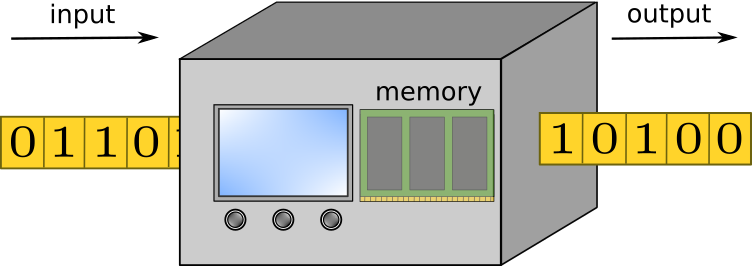
\includegraphics[width=0.7\textwidth]{images/transducer.png}
    \caption{A classical device simulating the ideal reference statistics of some KS-type experiment, consisting of sequential measurements. The device is fed a sequence of inputs (measurement choices) and produces outputs (measurement outcomes), based on its internal state prior to an input. The internal state of the device, which one can equate with a memory, stores relevant historical information about the past input-output process, on the basis of which the device generates the correct input-output statistics. After one input-output cycle, the device can update its memory state.}
    \label{fig:transducer}
\end{figure}

\begin{definition}[\cite{Barnett2015}]
An \emph{information transducer} is a tuple $(\mathcal{X},\mathcal{Y},\mathcal{S},\mathcal{T})$ where
\begin{itemize}
    \item $\mathcal{X}$, $\mathcal{Y}$ are the transducer's (finite) input and output alphabets,
    \item $\mathcal{S}$ is a (finite or countably infinite) set of internal memory states, and
    \item $\mathcal{T}\equiv\{p(S_{i+1}=s', Y_i=y\vert S_i = s, X_i=x)\}_{x,\thinspace y,\thinspace s,\thinspace s'}$ is the set of conditional ouput-transition probabilities.
\end{itemize}
More concretely, $p(S_{i+1}=s', Y_i=y\vert S_i = s, X_i=x)$ denotes the probability of the transducer outputting $y$ and transitioning to the internal state $s'$ after the $ith$ input-output cycle, conditioned on the input $x$ and internal state $s$.
\end{definition}

We require a valid classical model to produce statistics that are consistent with the infinite family of stochastic processes describing the quantum probabilities of the ideal reference experiment: $\{P(\oset{\leftrightarrow}{Y}|\oset{\leftrightarrow}{x})\}_{\oset{\leftrightarrow}{x}}$\thinspace, $\oset{\leftrightarrow}{x}$ being an instantiation of the input sequence $\oset{\leftrightarrow}{X}$.

Input-output transducers have been extensively studied within the field of computational mechanics. Of interest to us are memory-optimal classical models that produce the correct statistics $\{P(\oset{\leftrightarrow}{Y}|\oset{\leftrightarrow}{x})\}_{\oset{\leftrightarrow}{x}}$\thinspace. A transducer is memory-optimal if it stores the minimal amount of information about the past (in terms of number of bits) to make statistically correct future predictions. It has been shown that for stationary input-output processes there exists a unique memory-optimal transducer producing the correct statistics: the process' $\epsilon$-transducer \cite{Barnett2015}. The memory-optimal transducer does not store all information about the past $\oset{\leftarrow}{Z}$, as this may be highly redundant. In particular, the memory-optimal transducer does not differentiate between pasts that predict statistically identical futures. As such, the internal states of an $\epsilon$-transducer are given by the causal states of the process. 

\begin{definition}
Let $\oset{\leftarrow}{X}$, $\oset{\rightarrow}{X}$ denote the past and future stochastic input processes, respectively.
The \emph{causal states} $[\oset{\leftarrow}{z}]$ of an input-output process $\oset{\leftrightarrow}{Y}|\oset{\leftrightarrow}{X}$ are the equivalence classes on the set of pasts $\oset{\leftarrow}{z}$ with respect to the equivalence relation
\begin{equation*}
\oset{\leftarrow}{z}\;\sim_\epsilon\;\oset{\leftarrow}{z}'\;\mathrel{\vcentcolon\Leftrightarrow} \;P(\oset{\rightarrow}{Y}|\oset{\rightarrow}{X},\oset{\leftarrow}{Z}=\oset{\leftarrow}{z})= P(\oset{\rightarrow}{Y}|\oset{\rightarrow}{X},\oset{\leftarrow}{Z}=\oset{\leftarrow}{z}').
\end{equation*}
\end{definition}

\subsection{Memory-optimal classical simulation of quantum correlations}
In \cite{Cabello2018} it is shown that, for a ``causally complete" KS contextuality reference experiment, the causal states of the process' $\epsilon$-transducer correspond one-to-one to the possible quantum states $\{\ket{\Phi_{\oset{\leftarrow}{z}}}\}_{\oset{\leftarrow}{z}}$ the system can occupy after all past measurements $\oset{\leftarrow}{x}$. The assumption of causal completeness holds for many KS contextuality scenarios and in the following we will examine the odd $n$-cycle KS contextuality scenarios, in particular the KCBS scenario for $\text{n}=5$. In \cite{Cabello2018} the same analysis is performed for the Peres-Mermin (see Section \ref{sec:4dim}) and Yu-Oh (see Section \ref{sec:kcbs}) sets of measurements.

For all ideal odd $n$-cycle reference experiments, the number of possible post-measurement states tends to infinity when we increase the number of measurements in our sequence. However, the post-measurement states are not all equally probable. Figure \ref{fig:causalstates} illustrates this behaviour for the KCBS scenario $\text{n}=5$.

\begin{figure}
        %\centering
        \begin{subfigure}{0.5\textwidth}
            \centering
            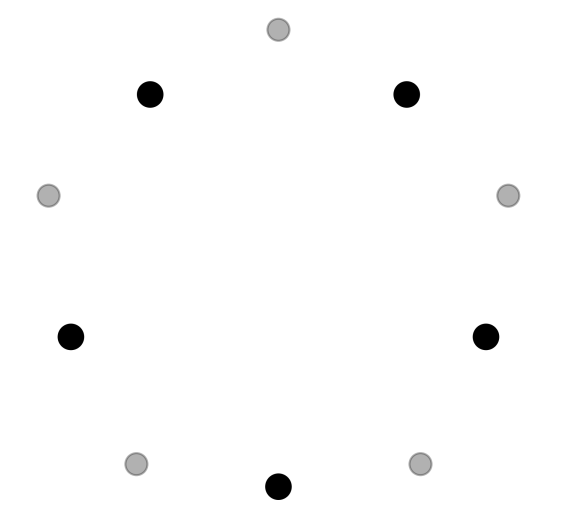
\includegraphics[width=0.8\textwidth]{images/n=5,mnts=1.png}
            \caption{one measurement}
        \end{subfigure}
        \hfill
        \begin{subfigure}{0.5\textwidth}
            \centering 
            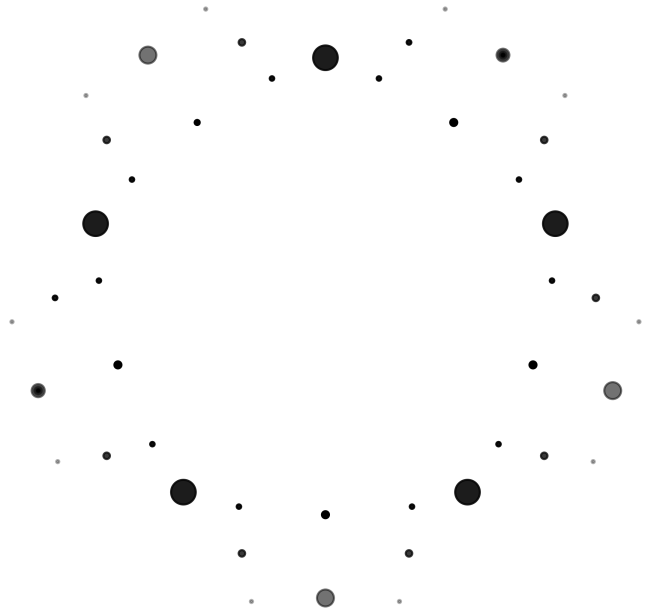
\includegraphics[width=0.8\textwidth]{images/n=5,mnts=3.png}
            \caption{three measurements}
        \end{subfigure}
        \vskip\baselineskip
        \begin{subfigure}{0.5\textwidth}
            \centering 
            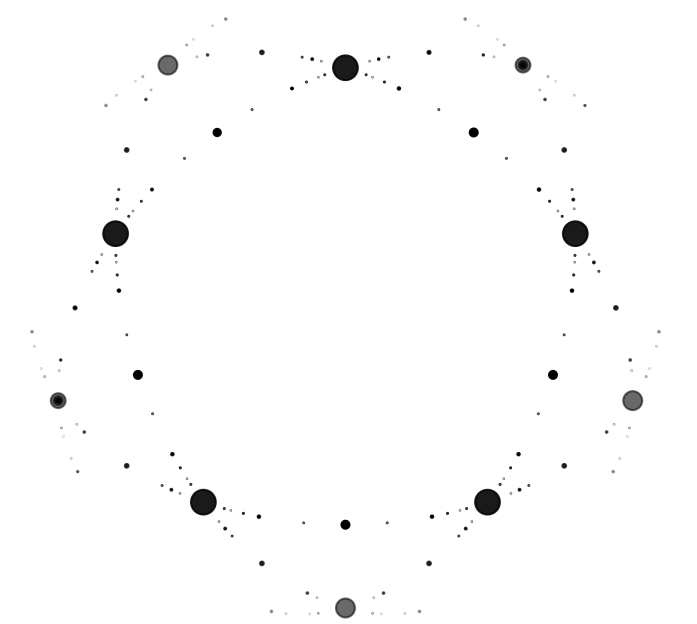
\includegraphics[width=0.8\textwidth]{images/n=5,mnts=5.png}
            \caption{five measurements}
        \end{subfigure}
        \hfill
        \begin{subfigure}{0.5\textwidth}
            \centering 
            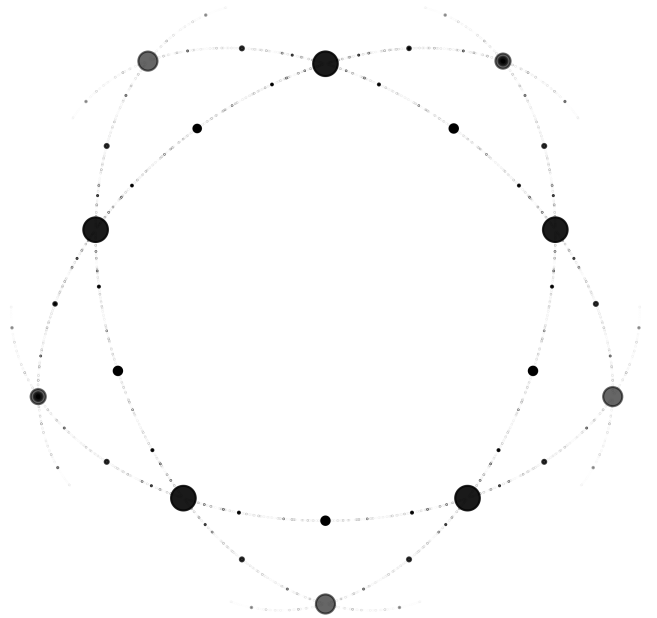
\includegraphics[width=0.8\textwidth]{images/n=5,mnts=10.png}
            \caption{ten measurements}
        \end{subfigure}
        \caption{Possible post-measurement quantum states after one, three, five, and ten measurements for the ideal KCBS experiment. The components of the post-measurement quantum states w.r.t.\ the standard qutrit basis are all real. The phases (signs) of the real qutrit states are chosen such that the corresponding vectors lie on a joint semisphere of $\mathbb{R}^3$. What is plotted are centered views of the three-dimensional plots along the negative x direction. As can be seen, the number of possible post-measurement states increases with the number of sequential measurements. The volume of a scattered point is proportional to the probability of the system being in that state after the measurements. The probability distribution over possible post-measurement quantum states becomes approximately stationary for large measurement sequences. The fact that all states lie on one of five semi-circles is a consequence of the compatibility structure of the five KCBS measurements. Analogous plots are obtained in \cite{Cabello2018} for the Peres Mermin and Yu-Oh KS contextuality scenarios.}
        \label{fig:causalstates}
    \end{figure}

Problematically, the process describing the ideal quantum experiment is not stationary, i.e.\ not invariant under translations in time, as can be seen from Figure \ref{fig:causalstates}. However, if we ``truncate" the process and consider only input-output cycles after sufficiently many initial measurements, the probability distribution over quantum states and by extension the stochastic process describing the experiment becomes stationary for all practical purposes. We only have a notion of the memory-optimal statistics-emulating classical model for the case of stationary processes. For this reason we will always consider the truncated input-output process, noting that the $\epsilon$-transducer's memory cost refers to the minimal number of bits needed to generate correct statistics, ignoring some of the initial behaviour. The true minimal number of memory bits a classical simulation requires to produce the correct statistics for all input-output cycles may therefore be greater. 

To numerically compute the memory cost, we consider all possible measurement sequences of a given length k. The statistical complexity of the process (RAM memory cost) is then the Shannon entropy $H=-\sum_ip_i\log_2p_i$ of the probability distribution over all achievable post-measurement quantum states after $k$ measurements, in the limit of $k\rightarrow\infty$ \cite{Cabello2018,Barnett2015}. Recall that this probability distribution becomes approximately stationary, reflected by the above expression converging. We find the number of bits (RAM) needed by a memory-optimal simulation of the ideal reference KCBS experiment to be just over 4. The statistical complexity thus exceeds the information carrying capacity $\mathcal{C}=\log_2(3)$ of the reference qutrit. In \cite{Cabello2018} the same qualitative behaviour is observed for the Peres-Mermin and Yu-Oh sets of measurements, both of which exhibit state-independent KS contextuality. 

An interesting feature we observe is that the memory cost of simulating the ideal reference experiment for odd $n$-cycle contextuality scenarios with $\text{n}\geq5$ odd increases with the number of exclusivity graph vertices $n$, as is shown in Figure \ref{fig:ncycleRAM}. However, this increase is only logarithmic. Furthermore, what does not change is the fact that, no matter the cycle length, we need to assume an upper bound on the unknown device's information carrying capacity in order to conclude quantumness. Additionally, we need to assume that each measurement device is used only once, requiring a potentially infinite supply, as otherwise the measurement device, and not the system whose information carrying capacity we bound, could retain memory about the past stochastic process.

\begin{figure}
        \centering
        \begin{subfigure}{\textwidth}
            \centering
            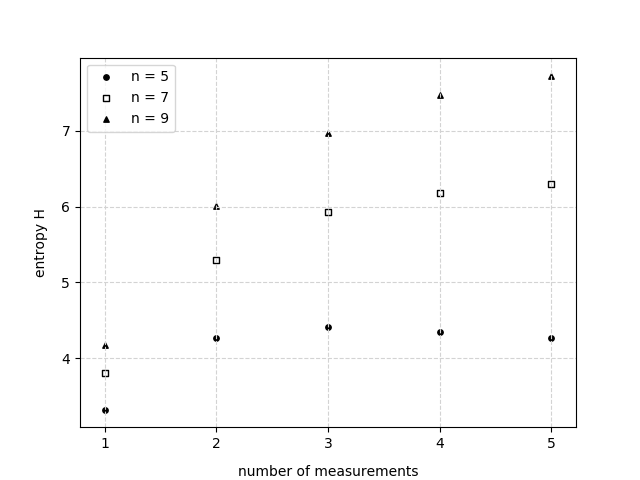
\includegraphics[width=0.7\textwidth]{images/allentropies.png}
            \caption{Plotted is the Shannon entropy of the probability distribution over all achievable post-measurement quantum states after a given number of measurements for the 5, 7, and 9-cycle KS contextuality scenarios. The probability distribution over possible post-measurement quantum states becomes approximately stationary for a sufficiently large number of measurements and the entropies thus saturate. This stationary limit of $H$ is the process' RAM memory cost, and it increases with an increasing cycle length}
        \end{subfigure}
        \vskip\baselineskip
        \begin{subfigure}{\textwidth}
            \centering 
            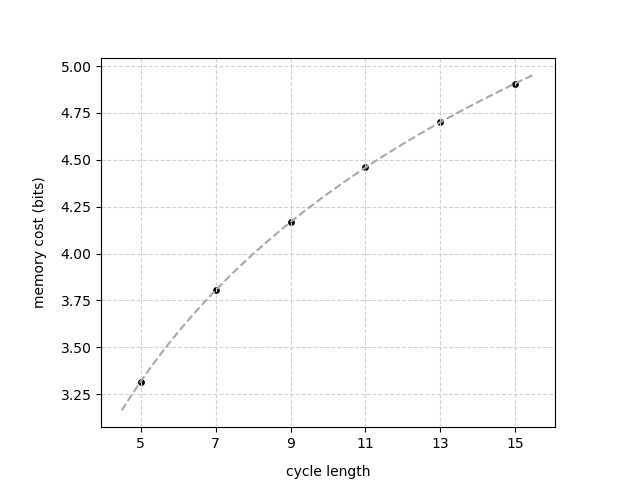
\includegraphics[width=0.7\textwidth]{images/memorycost.png}
            \caption{The RAM memory cost of classically simulating the ideal reference experiment for $n$-cycle KS contextuality scenarios increases logarithmically with the number of ideal measurements obeying cyclic compatibility that are performed.}
        \end{subfigure}
        \caption{The RAM memory cost of classically simulating the ideal reference experiment for odd $n$-cycle KS contextuality scenarios in terms of the cycle length $n$.}
        \label{fig:ncycleRAM}
\end{figure}


\subsection{Classical simulations dissipate heat}
\label{sec:landauer}
As advertised, let us briefly discuss the alternative approach to assuming an upper bound on the unknown device's information carrying capacity. It is based on Landauer's principle and we will make the following assumption \cite{Cabello2016}:
\begin{enumerate}
    \item sequential measurements can be chosen freely at random (as before),
    \item any classical simulation of the input-output process has limited memory
    \item Landauer's principle holds.
\end{enumerate}

First an intuitive description of how Landauer's principle aids us in certifying quantumness.
Assumptions 1 and 2 imply that any classical simulation must erase information during its operation: The simulation cannot know in advance the measurement sequence the experimenter chooses freely at random. Additionally, due to its finite capacity, the simulation's memory cannot contain instructions about what to do for all possible measurement sequences, i.e.\ the device cannot store in memory the internal states the system will be in for all possible measurement sequences. Therefore, the memory-bounded simulation has to erase memory bits, so it can store the updating historical information about the process, which enables it to emulate the ideal reference realization. Landauer's principle relates this erasure to a thermodynamical cost, meaning that the classical simulation will have to dissipate a minimal amount of heat to the environment for every measurement. If we do not detect this extra Landauer heat dissipated to the environment during measurement sequences, then we can be sure that our system is quantum, assuming that any adversary is bounded by finite memory $\dots$ in principle. The unit of extra Landauer heat emitted per measurement by a classical device is of the order $\sim k_B T$, rendering this method of certifying quantumness highly unrealistic. The following is a quantitative treatment of the intuition just presented.

It can be proven that the classical simulation of an input-output process that on average dissipates the minimal unit of heat per measurement is the process' memory-optimal $\epsilon$-transducer \cite{Cabello2016}. Consider the $\epsilon$-transducer of a stationary input-output process. The $\epsilon$-transducer is unifilar \cite{Barnett2015}, due to the causal structure of its internal states. Unifilar describes the property that the present internal state, input $x'$, and subsequent output $y'$ uniquely determine the next internal state of the machine. The subsequent internal state is the causal state $[\oset{\leftarrow}{z}']$ corresponding to the updated past input-output process $\oset{\leftarrow}{z}'$, where $\oset{\leftarrow}{z}'$ is the concatenation of $\oset{\leftarrow}{z}$ and $(x',y')$. Importantly, the reverse is generally not true \cite{Wiesner2012}. The present internal state, previous input, and previous output in general do not determine the previous internal state uniquely. This means that the memory-optimal simulation ``forgets" information about its previous internal state and is as such a logically irreversible computation \cite{Wiesner2012}.

Landauer's principle states that whenever classical information is processed in a logically irreversible manner, for example when erasing a classical bit of information, the entropy of the environment increases by a corresponding amount. For the erasure (setting to zero) of a classical bit this entropy increase is at least $\Delta S_{env}\geq -\Delta S_{sys} = -(0-k_B\log(2))=k_B\log(2)$. This entropy increase is related to the heat dissipated to the environment reservoir via $\Delta Q= (\Delta S)\thinspace T$, meaning that the minimal amount of dissipated heat for the erasure of a single classical bit is given by $\Delta Q = k_B T \log(2)$.

For the $\epsilon$-transducer that simulates the ideal reference statistics, the Shannon entropy 
\begin{equation}
I_{erased}=H(S_{t-1}\vert X_t,Y_t,S_t)
\end{equation} 
characterizes the amount of erased information for one step of the computation \cite{Wiesner2012}. The erased entropy can be re-written as $I_{erased}=H(S_t\vert X_t, S_{t-1})+I(S_t:X_t)$ \cite{Wiesner2012}, which simplifies to $I_{erased}=H(S_t\vert S_{t-1})$. Identifying the causal states of the optimal transducer with the post-measurement quantum states gives us an explicit expression for the erased information per measurement for odd $n$-cycle contextuality scenarios:
\begin{equation*}
I_{erased}= -\frac{1}{n} \sum_{s,(x,y)} \pi(s) \expval{P_x^y}{s}\thinspace\log_2\left(\frac{\expval{P_x^y}{s}}{n}\right),    
\end{equation*}
where we sum over all causal states $s$ and $(x,y)\in\{1,\dots,n\}\times\{0,1\}$. $\pi$ is the stationary probability distribution over the causal states and $\text{P}_x^y$ is the projector corresponding to the measurement-outcome pair $(x,y)$.

We find that any classical simulation that emulates the ideal KCBS experiment must erase at least $\sim 2.75$ bits for each measurement (in the stationary regime).
Therefore, the heat per measurement any classical simulation dissipates is at least $\sim 2.75\thinspace k_B\thinspace T \log(2)$. The heat dissipated by classical devices emulating higher order odd $n$-cycle scenarios increases with the cycle length $n$: By paying a price in terms of the number of ideal measurements satisfying cyclic compatibility we must implement, we can increase the minimal unit of heat that a classical simulation must dissipate per measurement cycle. Once again, this dependence is only logarithmic, as can be seen in Figure \ref{fig:erasedbits}.

\begin{figure}
    \centering
    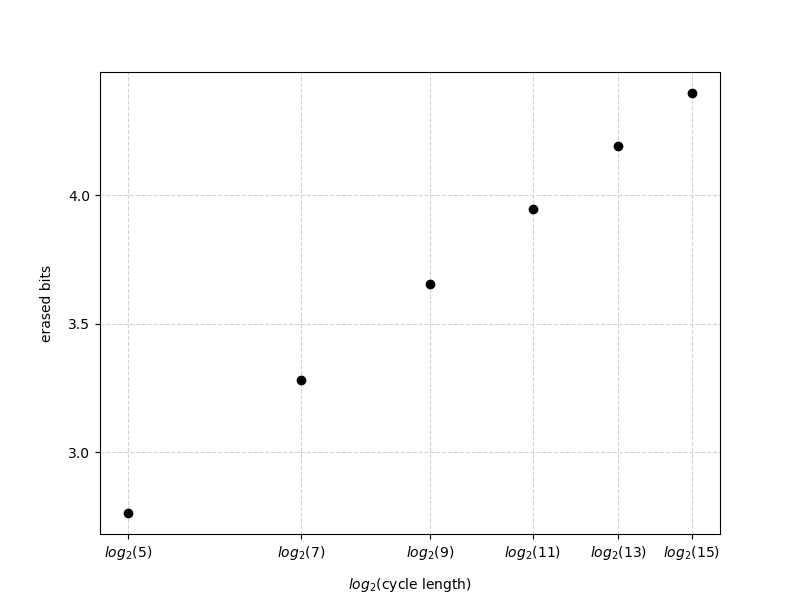
\includegraphics[width=0.7\textwidth]{images/erasedbits.png}
    \caption{The minimal number of bits a classical simulation of the ideal $n$-cycle reference experiment must erase per measurement, in terms of the cycle length $n$. The number of erased bits increases logarithmically with the cycle length.}
    \label{fig:erasedbits}
\end{figure}
